\batchmode
\makeatletter
\def\input@path{{/Users/Adam/Dropbox/Stat215A-2013/Labs/Lab2/Lab//}}
\makeatother
\documentclass[english]{article}\usepackage{graphicx, color}
%% maxwidth is the original width if it is less than linewidth
%% otherwise use linewidth (to make sure the graphics do not exceed the margin)
\makeatletter
\def\maxwidth{ %
  \ifdim\Gin@nat@width>\linewidth
    \linewidth
  \else
    \Gin@nat@width
  \fi
}
\makeatother

\IfFileExists{upquote.sty}{\usepackage{upquote}}{}
\definecolor{fgcolor}{rgb}{0.2, 0.2, 0.2}
\newcommand{\hlnumber}[1]{\textcolor[rgb]{0,0,0}{#1}}%
\newcommand{\hlfunctioncall}[1]{\textcolor[rgb]{0.501960784313725,0,0.329411764705882}{\textbf{#1}}}%
\newcommand{\hlstring}[1]{\textcolor[rgb]{0.6,0.6,1}{#1}}%
\newcommand{\hlkeyword}[1]{\textcolor[rgb]{0,0,0}{\textbf{#1}}}%
\newcommand{\hlargument}[1]{\textcolor[rgb]{0.690196078431373,0.250980392156863,0.0196078431372549}{#1}}%
\newcommand{\hlcomment}[1]{\textcolor[rgb]{0.180392156862745,0.6,0.341176470588235}{#1}}%
\newcommand{\hlroxygencomment}[1]{\textcolor[rgb]{0.43921568627451,0.47843137254902,0.701960784313725}{#1}}%
\newcommand{\hlformalargs}[1]{\textcolor[rgb]{0.690196078431373,0.250980392156863,0.0196078431372549}{#1}}%
\newcommand{\hleqformalargs}[1]{\textcolor[rgb]{0.690196078431373,0.250980392156863,0.0196078431372549}{#1}}%
\newcommand{\hlassignement}[1]{\textcolor[rgb]{0,0,0}{\textbf{#1}}}%
\newcommand{\hlpackage}[1]{\textcolor[rgb]{0.588235294117647,0.709803921568627,0.145098039215686}{#1}}%
\newcommand{\hlslot}[1]{\textit{#1}}%
\newcommand{\hlsymbol}[1]{\textcolor[rgb]{0,0,0}{#1}}%
\newcommand{\hlprompt}[1]{\textcolor[rgb]{0.2,0.2,0.2}{#1}}%

\usepackage{framed}
\makeatletter
\newenvironment{kframe}{%
 \def\at@end@of@kframe{}%
 \ifinner\ifhmode%
  \def\at@end@of@kframe{\end{minipage}}%
  \begin{minipage}{\columnwidth}%
 \fi\fi%
 \def\FrameCommand##1{\hskip\@totalleftmargin \hskip-\fboxsep
 \colorbox{shadecolor}{##1}\hskip-\fboxsep
     % There is no \\@totalrightmargin, so:
     \hskip-\linewidth \hskip-\@totalleftmargin \hskip\columnwidth}%
 \MakeFramed {\advance\hsize-\width
   \@totalleftmargin\z@ \linewidth\hsize
   \@setminipage}}%
 {\par\unskip\endMakeFramed%
 \at@end@of@kframe}
\makeatother

\definecolor{shadecolor}{rgb}{.97, .97, .97}
\definecolor{messagecolor}{rgb}{0, 0, 0}
\definecolor{warningcolor}{rgb}{1, 0, 1}
\definecolor{errorcolor}{rgb}{1, 0, 0}
\newenvironment{knitrout}{}{} % an empty environment to be redefined in TeX

\usepackage{alltt}
\usepackage[T1]{fontenc}
\usepackage[latin9]{inputenc}
\usepackage{geometry}
\geometry{verbose,tmargin=1in,bmargin=1in,lmargin=1in,rmargin=1in}
\usepackage{fancyhdr}
\pagestyle{fancy}
\setlength{\parskip}{\smallskipamount}
\setlength{\parindent}{0pt}
\usepackage{amsthm}
\usepackage{amsmath}

\makeatletter

%%%%%%%%%%%%%%%%%%%%%%%%%%%%%% LyX specific LaTeX commands.
\providecommand{\LyX}{L\kern-.1667em\lower.25em\hbox{Y}\kern-.125emX\@}

%%%%%%%%%%%%%%%%%%%%%%%%%%%%%% Textclass specific LaTeX commands.
\numberwithin{equation}{section}
\numberwithin{figure}{section}

\@ifundefined{date}{}{\date{}}
%%%%%%%%%%%%%%%%%%%%%%%%%%%%%% User specified LaTeX commands.
\pagestyle{empty} 

\makeatother

\usepackage{babel}
\begin{document}

\title{Lab 2 - Linguistic Survey\\
Stat 215A}


\author{Jonathan Fischer}
\date{October 7, 2014}

\maketitle


\section{Introduction}
In this report, we revisit the redwood data of Lab 1 to examine the effects of adding various smoothers to the temperature density and plots of temperature and humidity for a fixed time of day. For this exercise, we wish to observe the differences in performance among different kernel and parameter choices. 

The second element of the lab utilizes the lingual data collected by Bert Vaux in his 2003 Dialect Survey. In our treatment, we clean the data before examining a few questions geographically. To allow for better analysis, we convert the data from categorical responses to a sequence of 0's and 1's indicating the choices selected by respondents. This permits the use of PCA and subsequent K-means clustering based on projections to the principal axes. Optimal clustering seems to occur for K=3, and we observe groupings based in the northeast, south, and midwest/west. Perturbation by subsampling and different initial conditions for K-means produced identical clusters, engendering confidence in our results.

\section{Redwood Data}

\subsection{Temperature Density Estimates via Kernel Smoothing}

Our first task is to generate kernel density estimates of temperature based on the data obtained on the macroscope network. We used the cleaned data set from Lab 1 and aggregated over time and node id to get the entire temperature profile. Four kernels were considered for estimation--biweight, Epanechnikov, Gaussian, and rectangular. We examined the density estimates for five choices of the bandwidth, as shown in Figure 2.1. Smaller bandwidths produced excessively spiky densities, though an adjustment factor of 1 or greater mitigated this concern. The high bandwidths resulted in oversmoothing, more or less yielding gaussian distributions. This reflects the bias-variance tradeoff in which bandwidth positively correlates with bias but negatively correlates with variance (see Homework 2.) The smaller bandwidth estimators suggest a trimodal density with peaks at around 10, 15, and 20 degrees Celsius. All kernels performed similarly with the exception of the rectangular kernel, which gave unstable estimates highly dependent on the bandwidth. 

\begin{figure}
\begin{center}
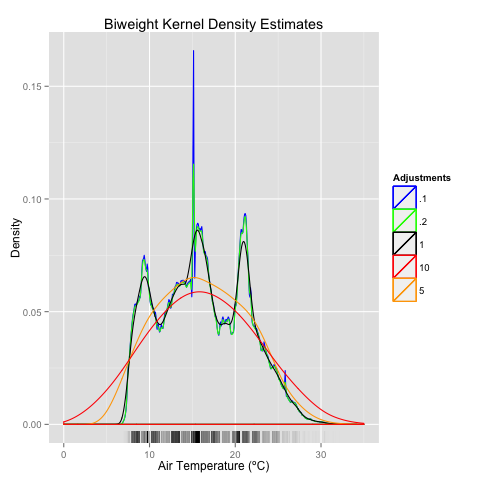
\includegraphics[scale = .4]{Temperature_Density_Biweight_Kernel.png}
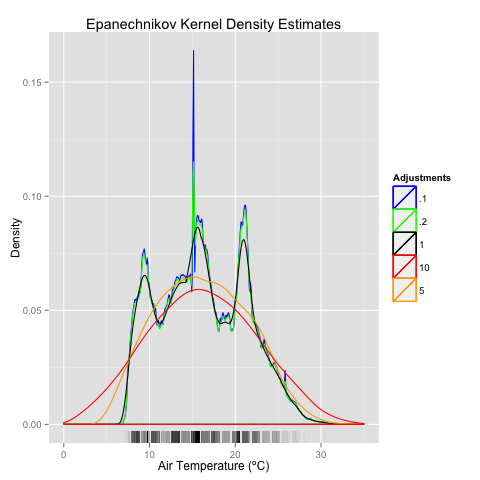
\includegraphics[scale = .4]{Temperature_Density_Epanechnikov_Kernel.png}
\end{center}

\begin{center}
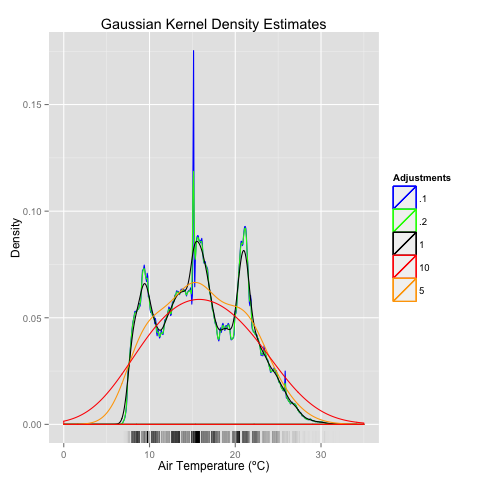
\includegraphics[scale = .4]{Temperature_Density_Guassian_Kernel.png}
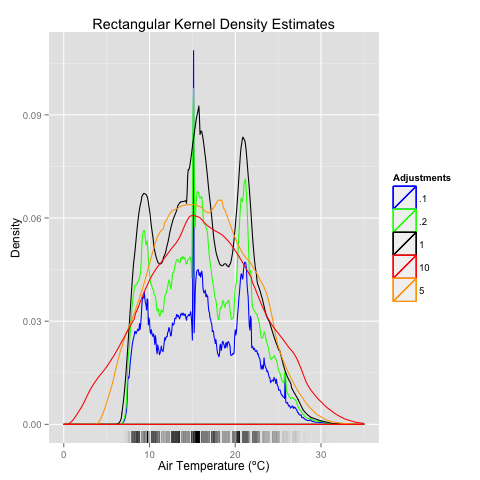
\includegraphics[scale = .4]{Temperature_Density_Rectangular_Kernel.png}
\end{center}
\caption{Kernel smoothed estimates of the temperature density for four different kernels. The rectangular kernel performs the worst while the others produce similar densities. Bandwidth = adjustment * .392 where .392 is the optimal bandwidth as calculated in R by bw.nrd0.}
\end{figure}

\subsection{Loess Smoothed Humidity vs Temperature}

To investigate Loess smoothing, we fixed the time of day at 10:05 AM and plotted humidity against temperature. We observe the negative correlation as before and fit Loess smoothers with polynomial degrees 0, 1, and 2 for four different spans. Here, the span is not an absolute bandwidth, rather it represents the proportion of points used in the smoother. For example, a span of .25 means we take the x closest points where x/n = .25 and n is the number of observations. Thus changing this value is akin to varying the bandwidth. Figure 2.2 shows the results. The degree 0 smoother does rather poorly compared to the higher degree versions as it is too flat for all spans. The degree 1 and 2 smoothers behave similarly, though the second-degree fit seems subtly more consistent across spans. As in the KDE plots, higher spans give a smoother trend while lower ones are more sensitive to the local behavior. 

\begin{figure}
\begin{center}
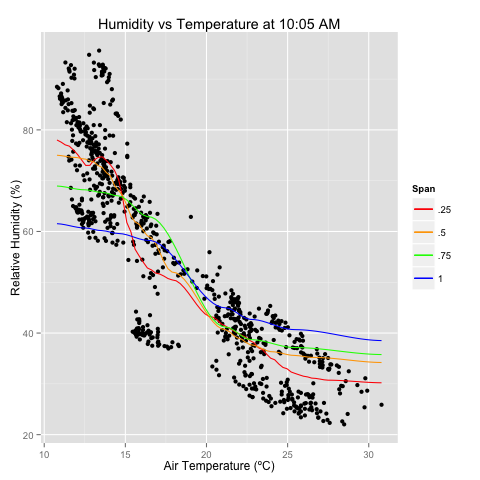
\includegraphics[scale = .4]{Humidity_Temperature_Loess_0.png}
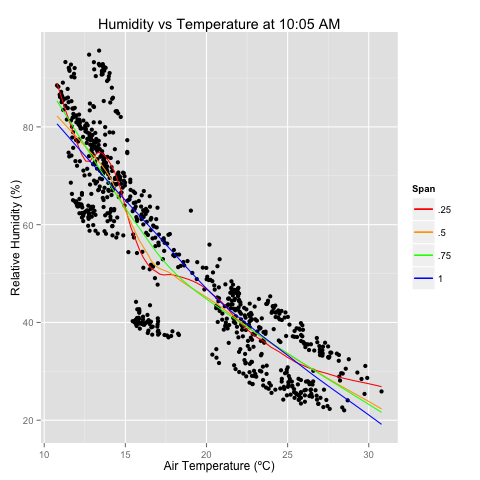
\includegraphics[scale = .4]{Humidity_Temperature_Loess_1.png}
\end{center}

\begin{center}
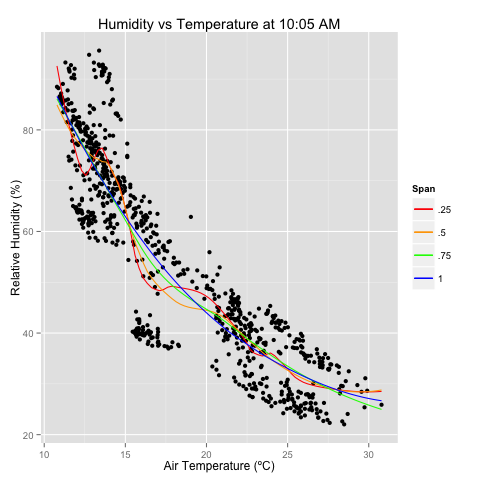
\includegraphics[scale = .4]{Humidity_Temperature_Loess_2.png}
\end{center}
\caption{Upper Left: Degree 0 Loess smoother. Upper right: Degree 1 Loess smoother. Bottom: Degree 2 Loess smoother. The second degree smoother produces more consisten results, but the degree one gives similar trends.}
\end{figure}

\section{Linguistic Data}

\subsection{Data quality and cleaning}

Each row of the data contains a participant's answers and each column corresponds to a different question. The entries are categorical variables that give the responses in the form of numbers where each number is associated with a specific answer. There were initially 47471 participants and 67 questions considered. Since we want to eventually generate maps using latitude and longitude, we began by removing all rows for which a latitude and longitude were not present. This was a total of 1020 respondents. Several systematic reasons for the missing coordinate data were considered, including zip codes starting with 0 and outdated zip code databases. Investigation of these possiblities yielded no improvement. Additionally, some participants answered few of the questions and were removed. We set a cutoff of 20 missing answers. This left us with 45107 observations. While they were included in the data for clustering, any points corresponding to locations in Alaska and Hawaii were removed for plotting. The latitude and longitude columns were separated from the response columns before encoding to binary variables since that procedure would not work if they remained. Furthermore, they were not readded until clustering was complete since PCA and the clusters would be influenced by the presence of location data and we would likely get geographic clusters by default.

Having the data in categorical form was sufficient for the EDA as it allowed for plotting and tracking how often responses were recorded together. However, further analysis required a transformation into binary variables as described in the lab's prompt. This was accomplished by defining a function based on model.matrix and applying it to each row of the data. The intercept columns were then removed to give a set of 468 binary response variables where a 0 indicates that answer was not chosen and a 1 says the opposite. 

\subsection{Exploratory Data Analysis}

Our EDA began with maps of the US overlaid with responses by latitude and longitude. Each point is colored by the responder's answer. For each question only the popular choices were included to prevent overplotting. The included plots correspond to the most important questions as measured by the loadings on the first 3 principal components. These are the plural second person, name for athletic shoes, and name for a water fountain questions. In Figure 3.1, the south is shown to strongly prefer using "y'all" while the rest of the nation favors "you", "you all", or "you guys" with no clear geographical trend among them. Figure 3.2 illustrates the divide in usage of "sneakers" and "tennis shoes." The northeast refers to the shoes in question as sneakers while the remainder of the country uses tennis shoes. In both examples, we see south Florida's behavior mimicking that of the northeast, perhaps as a consequence of the large number of transplants in the region. The final of our EDA plots, Figure 3.3, shows the geographic separation between the terms "water fountain" and "drinking fountain," with "drinking fountain" only being common in parts of the midwest and on the west coast. Considering these plots together, we note that each one defines a group. In fact, these correspond nicely to the clusters output by PCA and K-means. 

To look at the relationship between a pair of questions, we examine the second person plural and shoes questions. We calculated the frequencies of observing pairs of answers together and on their own and then computed the conditional probabilities of observing an answer to one question given the response of the other. To lower the dimensionality, we combined "you", "you all" and "you guys" into the category "you" for these calculations.

\begin{table}
\caption{Conditonal Probabilities}
\begin{center}
  \begin{tabular}{| c | c |}
    \hline
    P(TS|You) = .54 & P(Sneakers|You) = .46 \\ \hline
    P(TS|Y'all) = .73 & P(Sneakers|Y'all) = .27 \\ \hline
    P(You|TS) = .75 & P(You|Sneakers) = .87 \\ \hline
    P(Y'all|TSl) = ..25 & P(Y'all|Sneakers) = .13 \\ \hline
  \end{tabular}
\end{center}
\end{table}

From these probabilites we note that people who say sneakers are very unlikley to also say y'all (and vice versa). Since most people across two regions, say some variant of "you", conditioning on it doesn't really refine our ability to predict a person's shoe preference. Conditioning on shoes always suggests a high chance of observing "you" due to the much larger marginal probability of "you" because fewer samples come from the south than the collective rest of the nation.

We can follow a similar procedure to find the conditional probabilities with different combinations of responses for the three questions illustrated in Figures 3.1-3.3. This is a bit more involved since the number of possible combinations increases quickly with the number of questions, so it is an infeasible solution to analyze many questions. Furthermore, the separating the data when we have many questions to consider may lead to abnormally small sample sizes and yield imprecise results. 

\begin{figure}
\begin{center}
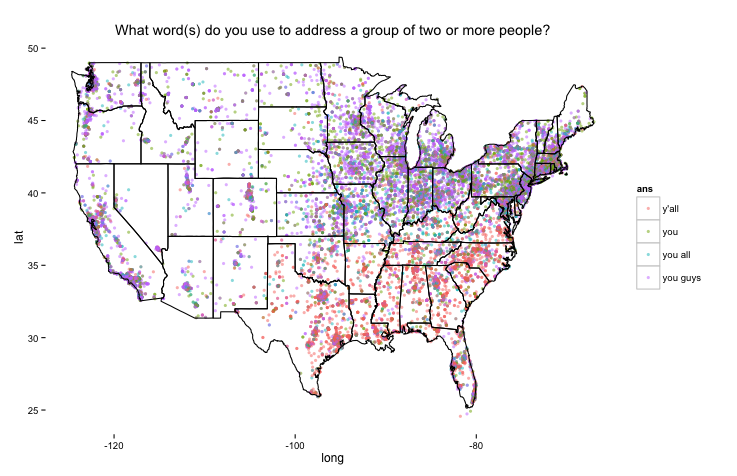
\includegraphics[scale = .5]{Rplot1.png}
\end{center}
\caption{Most popular ways to address a group of people mapped by latitude and longitude. Y'all is popular in the south, but the other choices are evenly spread across the rest of the country.}
\end{figure}

\begin{figure}
\begin{center}
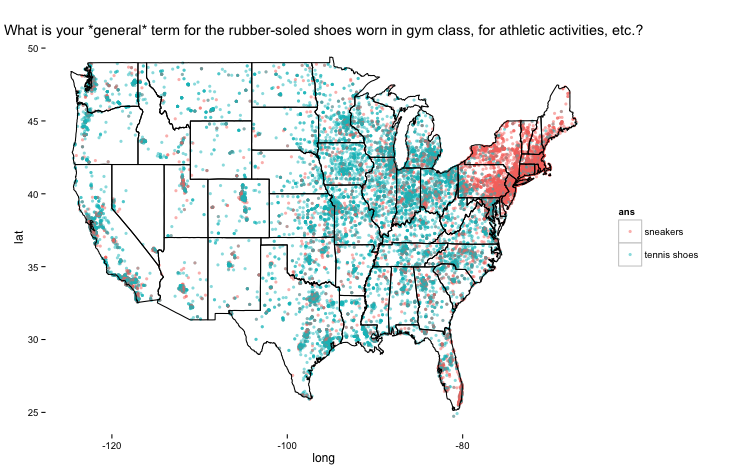
\includegraphics[scale = .5]{Rplot2.png}
\end{center}
\caption{Mapped responses for tennis shoes/sneakers. The northeast is the only region to prefer sneakers.}
\end{figure}

\begin{figure}
\begin{center}
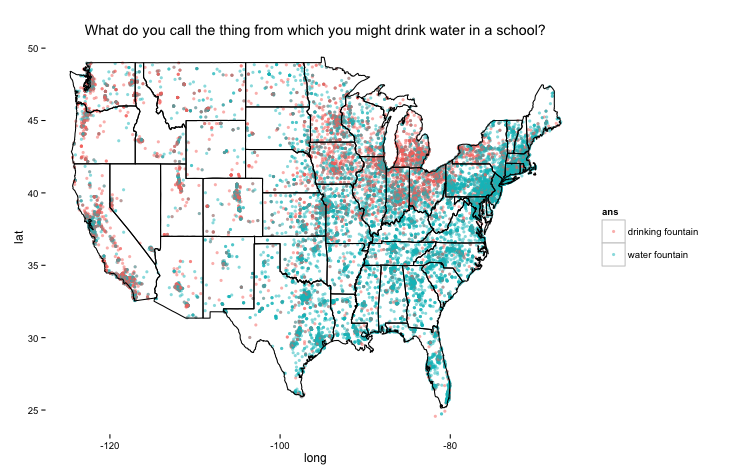
\includegraphics[scale = .5]{Rplot3.png}
\end{center}
\caption{Map of water/drinking fountain usage. The upper midwest and west coast show a preference for drinking fountain while everyone else says water fountain.}
\end{figure}


\section{Dimension reduction methods}

With the data expanded into a binary format, we were prepared to perform a PCA. We chose to use the centered analysis after comparing the outcomes of the centered and uncentered computations. In the uncentered case, while the first PC accounted for most of the variance, it gave no information on clusters and was dominated by the projections of the means. Centering gave a more meaningful PC in the context of differentiating amongst points. Scaling was not employed since all variables are on the same units and have the same support. 

\begin{figure}
\begin{center}
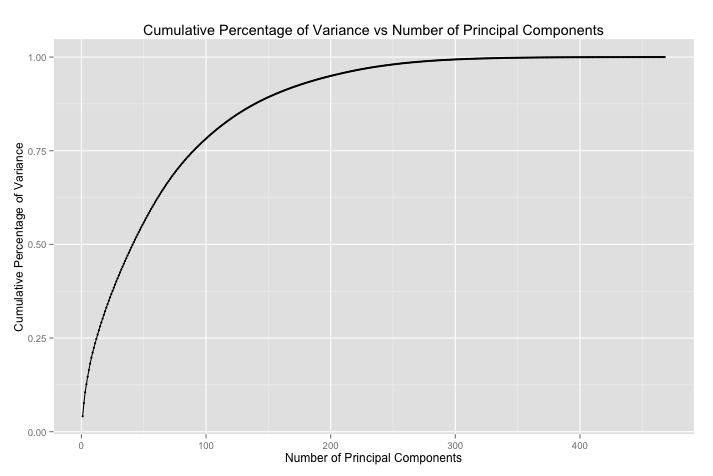
\includegraphics[scale=.3]{cumulativevariance.png}
\end{center}
\caption{Cumulative variance as a function of the number of principal components.}
\end{figure}

Figures 4.2-4.4 depict the projections of data onto pairwise combinations of the principal axes for the first three principal components. The left plot in each figure illustrates the projections without cluster annotation while the right sides are colored on the basis of the cluster assigned by K-means with K=3. We see differentiation occurs in the plane defined by the first two principal components with the division characteristic of K-means. The combination of these plots give us an idea of the density of points in PC space and also the spatial relationship of the clusters in this projection. Essentially, it seems the first principal component separates the northeast, while the second further distinguishes the south. Since the midwest/west and south clusters are not differentiated by the first PC, we may expect there to be more geographic overlap between these clusters than the other possible pairs. 

\begin{figure}
\begin{center}
\includegraphics[scale = .3]{PCA12bw.png}
\includegraphics[scale = .3]{PCA12c.png}
\end{center}
\caption{Scatter plot of projections onto the first and second principal component axes with and without annotation of K-means defined clusters.}
\end{figure}

\begin{figure}
\begin{center}
\includegraphics[scale = .3]{PCA13bw.png}
\includegraphics[scale = .3]{PCA13c.png}
\caption{Scatter plot of projections onto the first and third principal component axes with and without annotation of K-means defined clusters.}
\end{center}
\end{figure}

\begin{figure}
\begin{center}
\includegraphics[scale = .3]{PCA23bw.png}
\includegraphics[scale = .3]{PCA23c.png}
\end{center}
\caption{Scatter plot of projections onto the second and third principal component axes with and without annotation of K-means defined clusters.}
\end{figure}

\begin{figure}
\begin{center}
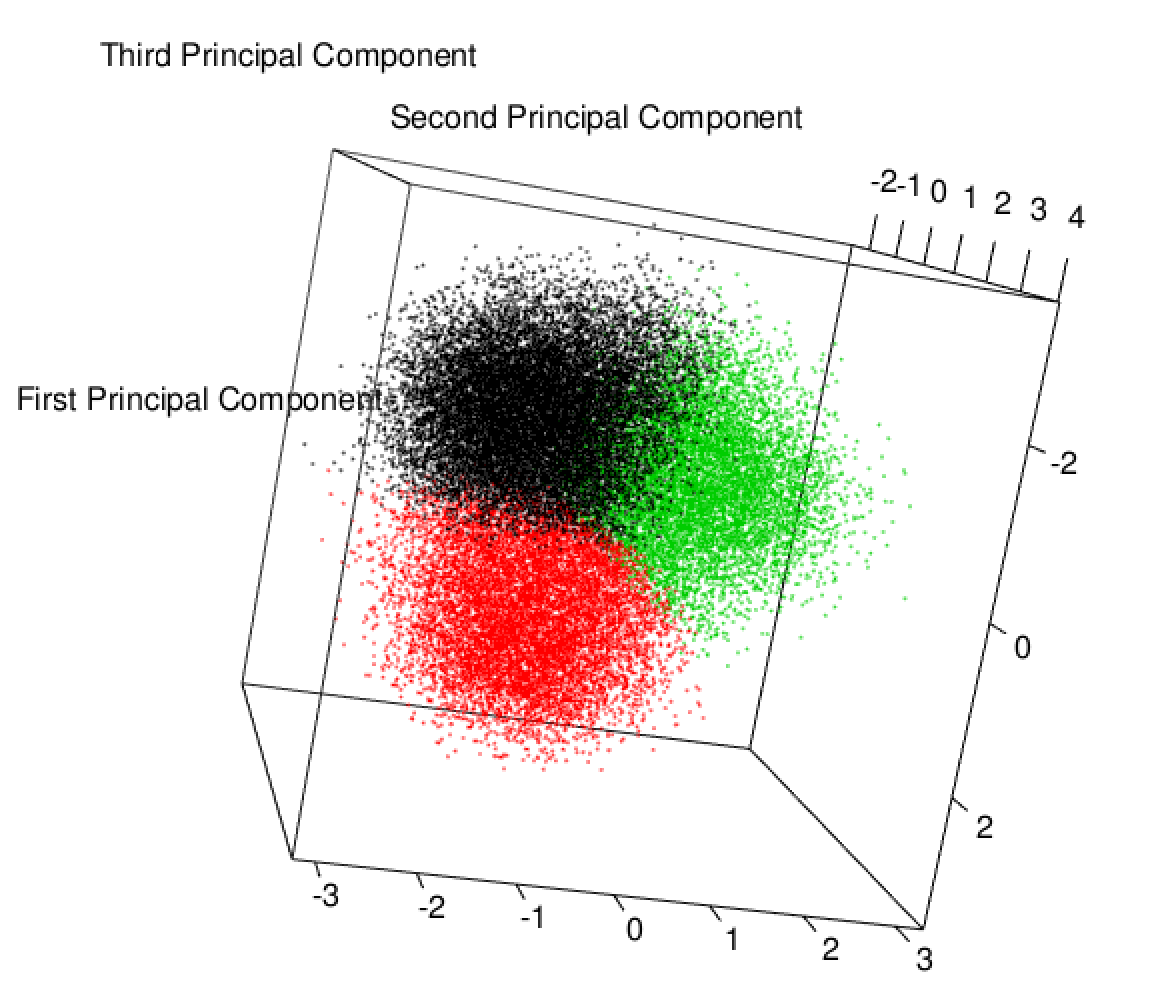
\includegraphics[scale = .3]{PCA3DScatter.png}
\caption{Screenshot of projection to first three principal axes with cluster coloring.}
\end{center}
\end{figure}

Based on the plots presented in the EDA section, K-means was first run for K=3. The result is Figure 4.6, in which we observe 3 clusters centered in the northeast, south, and midwest/west. The northeast cluster seems fairly dense in regions where it is common, dominating from Pennsylvania to Maine and the Miami region. There is a small overlap between the northeast and south clusters in the Pittsburgh area as well as in Maryland. On the other hand, there is quite a bit of mixing in the lower Great Lakes and Midwest, with Ohio, Indiana, Illinois, and Missouri having many points in both clusters. This aligns with our previous analysis of the discriminative power due to the first PC. The clustering was done using the first 3 PC, accounting for a little over 10 percent of the variance. This seems small, but we found no significant improvement in clustering when more PC's were included.

\begin{figure}
\begin{center}
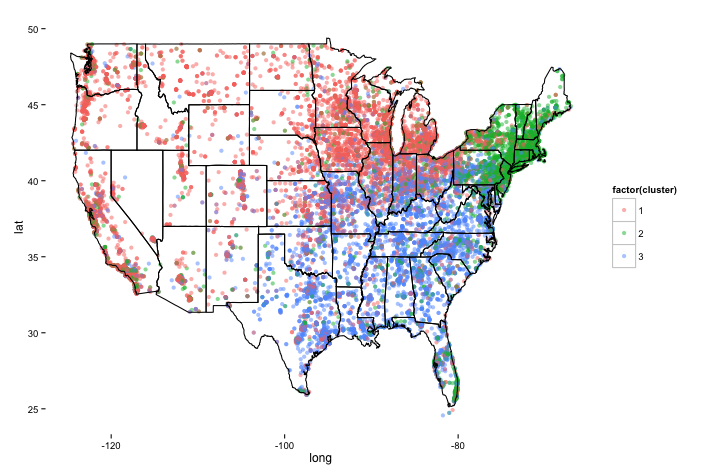
\includegraphics[scale=.5]{clusters.png}
\end{center}
\caption{Responders mapped onto USA and colored by K-means generated clusters with K=3. We see 3 geographically well-defined clusters--northeast, south, and midwest/west.}
\end{figure}

Having found three distinct clusters, we tried clustering again with K=4 to see if we could achieve differentiation among the midwest and western regions. Figure 4.7 shows that this fails to occur as members of clusters 3 and 4 are scattered throughout was was previously one cluster with no discernable geographic trend. In fact, even when all PC's were included, the final clusters were the same, so we concluded that the clustering with K=3 was the appropriate choice. 

Additional clustering methods such as EM on Gaussian mixtures and HDP were considered, and the EM algorithm was run using the implementation emcluster in the package EMCluster (see Figure 6.1). Interestingly, even when a mixture of 3 Gaussians was specified, only two clusters had a substantial number of points; these were the northeast/south and midwest/west. This behavior could be due to the the parametric assumptions imposed on the model in the EM treatment or the higher density of points in the west/midwest cluster due to the number of respondents from those areas. An HDP clustering algorithm that could detect the number of clusters (under the constraints of a hyperparameter penalizing the creation of new clusters) was not implemented but it would be interesting to do so. Hiearchical clustering for a suitable distance metric (L1?) could support the hypothesis that the northeast cluster is the 'most different' among the 3 observed.

By noting the greatest components of the eigenvectors of our rotation matrix, we can infer which responses have the largest impact in terms of separating or failing to separate clusters. Included in this list are the three questions discussed previously, and the table below indicates whether they distinguish a region or exhibit a large amount of similarity across regions. Maps for these questions were generated, and are not included in this report due to length limitations. 

\begin{table}
\caption{Subset of questions/responses and their geographic trends.}
\begin{center}
  \begin{tabular}{| c | c | p{5cm}  | p{3cm} |}
    \hline
    Question No. & Description & Notes & Discriminative? \\ \hline
    50 & 2nd Person Plural & Y'all in south, even split among you, you all, you guys elsewhere & Yes \\ \hline
    56 & Use of anymore & Acceptable in midwest save MN, WI, MI. Lots of mixing in these states, however. & Blurs midwest and south.  \\ \hline
    68 & Maternal grandmother & Other is widespread but leads in the south. Grandma also very common. Nana only in northeast. & Yes \\ \hline
    73 & Tennis Shoes/Sneakers & Sneakers in S. FL and northeast from eastern PA through ME. Tennis shoes otherwise. & Yes\\ \hline
    76 & catty/kitty-corner & Kitty-corner in west and upper midwest as well as NY and New England. Fairly separate. & Yes\\ \hline
    79 & freeway/highway & Highway almost everywhere. Cities in CA favor freeway. & No\\ \hline
    89 & coleslaw & Slaw is OK in south into lower midwest. & Continuum in OH, IN, IL \\ \hline
    98 & by/on accident & By is predominant everywhere. & No \\ \hline
    99 & road parallel to highway & Large amount of mixing but there is some separation that helps distinguish the midwest and west. & Blurs south with other regions \\ \hline
    103 & water/drinking fountain & Drinking fountain near great lakes and in the west. Lots of overlap in rust belt and bay area. & Some, but doesn't completely separate midwest. \\ \hline
    105 & soda/pop/coke & Soda in northeast, coke in south, pop in midwest and pacific NW, soda in CA. & Yes, but doesn't perfectly match clusters \\ \hline
    106 & term for TP'ing & Higher presence of rolling in south and toilet papering in northeast than elsewhere. & Yes \\ \hline
    120 & shotgun & Shotgun wins. & No \\ \hline
  \end{tabular}
\end{center}
\end{table}

\begin{figure}
\begin{center}
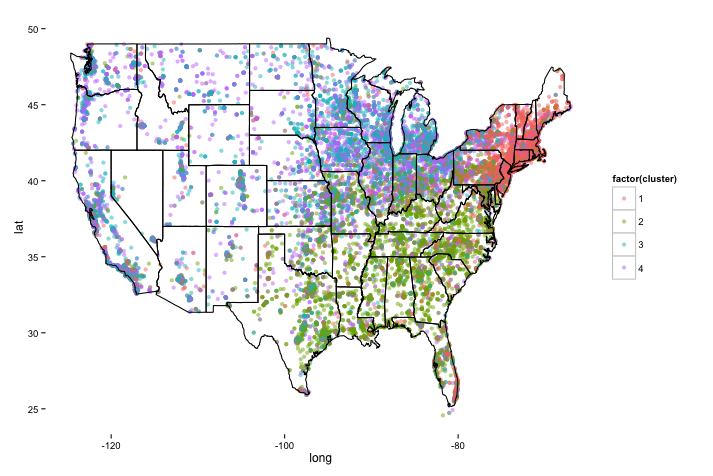
\includegraphics[scale=.5]{pcamap4clusters.png}
\end{center}
\caption{Responders mapped onto USA and colored by K-means generated clusters with K=4. The south and northeast clusters remain but two clusters are mixed throughout the west/midwest. This suggests 3 clusters was more appropriate.}
\end{figure}

\begin{verbatim}
Animation of 3D scatterplot of PC: http://youtu.be/-qgCEqmbsO4
Animation containing maps for all analyzed questions: http://youtu.be/FuRNZofyJgs
\end{verbatim}


\section{Stability of findings to perturbation}
To test whether our finding of 3 distinct regional clusters was stable, we took random subsamples of the data and re-ran the analysis. Each subsample consited of 10000 points and the indices were chosen uniformly. Figure 5.1 displays the resulting plot for one such subsample, which looks like Figure 4.6 but with fewer mapped points and a new color permutation. All subsamples tested produced the same picture, suggesting the clusters are fairly robust. 

Since the linguistic regions arise in Figures 3.1-3.3, we also conducted the entire analysis with only these three questions rather than the full set of 67. We see the outcome in Figure 5.2. This strategy seems to capture the geographic differences somewhat well, though there is more mixing than when the full data are used. This is particularly apparent in Missouri, which has many "southern" respondents in the map using the full data but not many in this realization. This is because not many people chose "y'all" in question 50. The presence of the same three clusters, give or take a few locations, supports the strength of our findings. 

The final test of stability we performed was altering the starting points for K-means. Each time the function is invoked in R, random points are chosen as the starting coordinates for the clusters. We ran K-means several times, allowing it to uniformly select the centers at which to start. In each case, the results were identical once we accounted for permutations of the cluster numbers. Additionally, we ran a simulation with centers at (1,0,0), (0,1,0), (0,0,1). This similary produced the same clustering outputs.

\begin{figure}
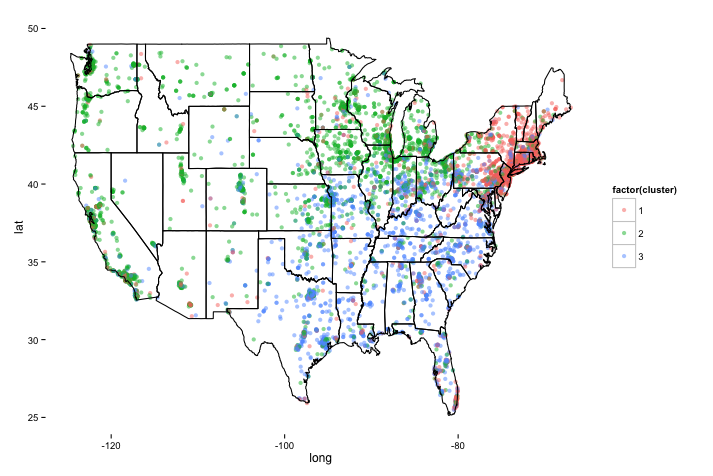
\includegraphics[scale=.4]{pcasubsample.png}
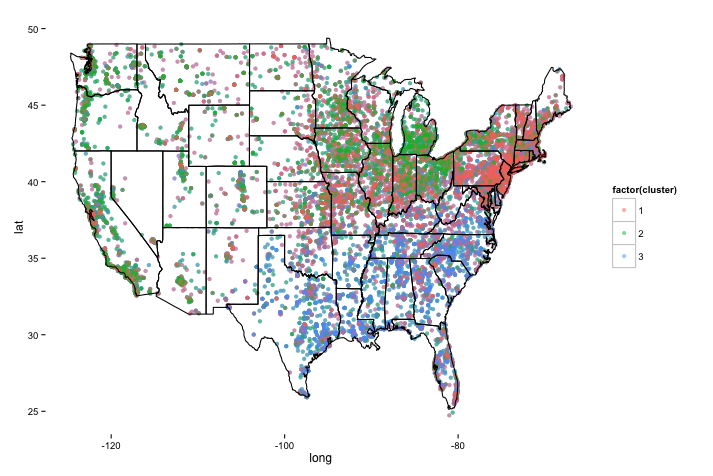
\includegraphics[scale=.4]{pca3questions.png}
\caption{Left: The results of PCA and clustering with K=3 with a random subsample of 10000 points. The same geographic clusters arise. Right: The results of PCA and clustering with K=3 where the data have been reduced to responses to questions 50 (not y'all/y'all), 73 (sneakers/tennis shoes), and 103 (water/drinking fountain). There is more overlap in the clusters than when the full data are used, but we still see the distinct geographic pattern.}
\end{figure}



\section{Conclusion}
This report discussed the impact of smoothing parameters on kernel density estimation and Loess smoothing, supporting the theorectical result that increasing bandwidth decreases variance but increases bias while decreasing bandwidth does the opposite. In our second component, we cleaned and analyzed dialect survey data consisting of 67 questions answered by 47471 participants. Our work suggests three separate linguistic clusters based on lexical differences, geographically centered in the northeast, south, and combination of the midwest/west. These findings are stable under the perturbation analyses performed, though the failure of the Gaussian mixture model using EM would be interesting to investigate. We were surprised to see the discriminative power of the first few PC given their small cumulative proportion of the variance, but adding more PCs did not alter the clusters. Given our anecdotal experience, we anticipated differentiation among the northeast, south, and midwest. Conversely, it was unexpected to see the west and midwest grouped into one cluster, though the maps for many questions bore this out upon examination. 

\begin{figure}
\begin{center}
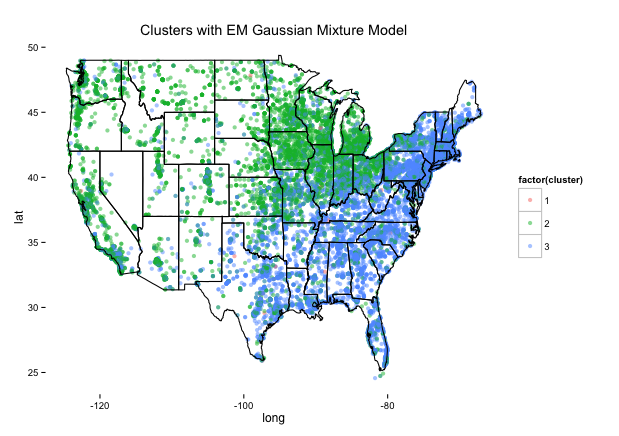
\includegraphics[scale=.5]{EMclusters.png}
\end{center}
\caption{The results of PCA and clustering with EM Gaussian mixture model and 3 clusters. We see only two clusters really arise as the northeast and south have been merged.}
\end{figure}


\end{document}
